	\subsection{Maximum Flow Problem}
	\begin{defn}[Directed Graph]
		A \textbf{directed graph} is an ordered pair with a set of vertices $V(G)$ and an arc set $A(G) \subseteq \binom{V}{2}$ containing directed edges.
	\end{defn}

	\begin{marginfigure}
		Let $G = (V,A)$ be a directed graph,
		\begin{itemize}
			\item $|V(G)| = n$
			\item $|A(G)| = m$
		\end{itemize}
	\end{marginfigure}

	\begin{defn}[Directed Path]
		A \textbf{directed path} in a directed graph is a path in which every edge is traversed from tail to head.
	\end{defn}

	\begin{defn}[Directed Neighborhood]
		$\delta^+(X)$ is the set of arcs with a tail in $X$ and a head in $V(G) - X$. In contrast, $\delta^-(X) = \delta^+(V(G)-X)$.
	\end{defn}

	\begin{defn}[Capacity]
		Every arc $a = (i,j)$ in $A(G)$ has an integral\footnote{$u_a > 0$ for all arcs $a \in A(G)$. If an arc does not exist, we can assume that it has capacity zero.} \textbf{capacity} $u_a = u_{ij}$, which is the maximum amount that flows through it.
	\end{defn}

	\begin{defn}[Flow]
		Let $G = (V,A)$ be a directed graph. A \textbf{flow} $f$ from a source $s$ to a sink $t$ is a function $f: A(G) \rightarrow R^+$ that satisfies,
		\begin{itemize}
			\item $0 \leq f_a \leq u_a$ for all $a \in A(G)$
			\item $\sum_{a \in \delta^-(v)} f_a = \sum_{a \in \delta^+(v)} f_a$ for all $v \in V(G) - \{s,t\}$
		\end{itemize}
		\noindent The first condition, capacity constraints, states that the flow on an arc $a \in A(G)$ is non-negative and at most its capacity. The second condition, flow conservation, states that the inflow of a vertex $v \not\in \{s,t\}$ equals its outflow.
	\end{defn}

	\begin{defn}[Flow Value]
		Assume that $\delta^+(t) = \delta^-(s) = \emptyset$. Then the \textbf{value} of a flow $f$ is the quantity of flow that reaches the sink,
		\[|f| = \sum_{a \in \delta^-(t)} f_a = \sum_{a \in \delta^+(s)} f_a\]
	\end{defn}

	\begin{defn}[Maximum Flow]
		Let $G = (V, A)$ be a directed graph. The \textbf{maximum flow problem} is the problem of finding $f^*$, where,
		\[
		  f^* = \max \Set{ \sum_{a \in \delta^-(t)} f_a \ | \begin{array}{l}
		    \sum_{a \in \delta^-(v)} f_a = \sum_{a \in \delta^+(v)} f_a \quad \forall v \in V(G) - \{s,t\} \\
		    0 \leq f_a \leq u_a \quad \forall a \in A(G)
		  \end{array}}
		\]
	\end{defn}

	\begin{defn}[Augmenting Path]
		An $(s-t)$ path $P$ is \textbf{augmenting} if\footnote{\begin{center}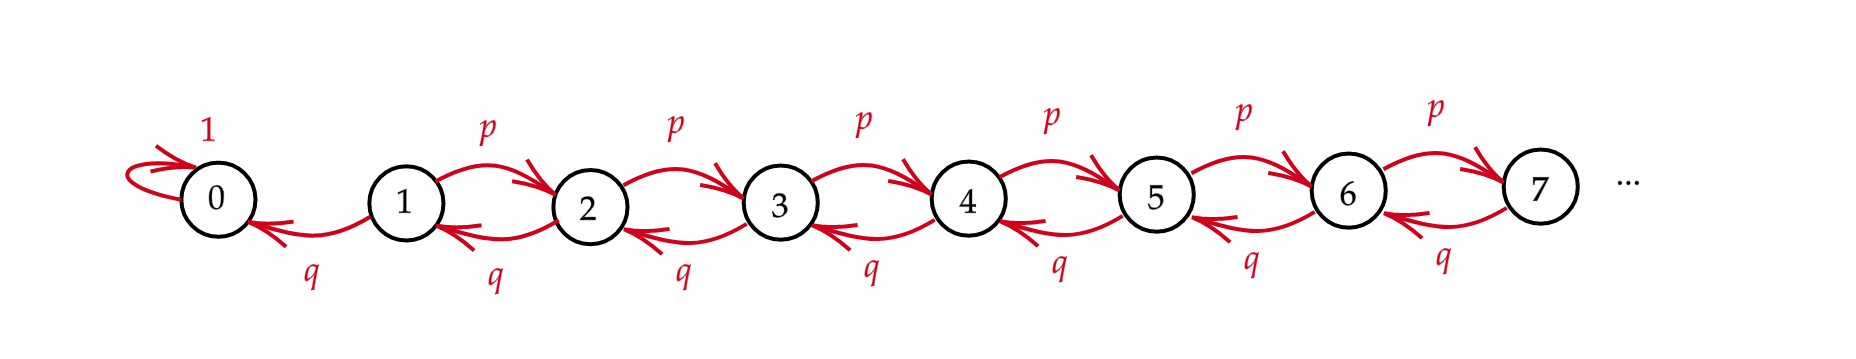
\includegraphics[width=0.5\textwidth]{fig-27.png}\end{center}},
		\begin{itemize}
			\item $f(a) \leq u_a - 1$ for every arc $a$ used in the forward direction of $P$
			\item $f(a) \geq 1$ if $a \in A(P)$ is traversed in the backwards direction
		\end{itemize}
		\noindent Equivalently, $P$ is a directed path from $s$ to $t$ in the residual network $G_f$.
	\end{defn}

	\begin{defn}[Bottleneck Capacity]
		The \textbf{bottleneck capacity} of an augmenting path $P$ with respect to a flow $f$ is the maximum amount $b(P, f)$ that we can increase the flow along $P$ by,
		\[
		b(P, f) = \min \Set{ \min_{\tiny\begin{array}{c} (i,j) \in A \\ i \rightarrow j \end{array}} u_{ij} - f_{ij}, \min_{\tiny\begin{array}{c} (i,j) \in A \\ i \leftarrow j \end{array}} f_{ij}}
		\]
	\end{defn}

	\begin{defn}[Residual Graph]
		Let $G = (V,A)$ be a directed graph, and suppose that $f$ is a flow on $G$. The \textbf{residual graph} $G_f$ satisfies,
		\begin{itemize}
			\item $\exists a_1 \in A(G_f)$ such that $u_{a_1} = u_a - f_a$
			\item $\exists a_2 \in A(G_f)$ such that $u_{a_2} = f_a$
		\end{itemize}
		\noindent for all $a \in A(G)$.
	\end{defn}

	\begin{rmk}
		The bottleneck capacity of a path is the minimum capacity of an arc in the corresponding directed path in the residual graph.
	\end{rmk}

	\begin{defn}[Ford-Fulkerson]
		Let $G = (V,A)$ be a directed graph. The following algorithm produces a maximum flow $f^*$,
	\begin{algorithm}
	  \caption{Ford-Fulkerson}\label{fordfulk}
	  \Comment{$f$ is globally given, and initially set to $0$.}
	  \Function{Augment($P, f$)}{
	  	$b \assign \text{bottleneck capacity $b(P,c)$}$\;
	    \ForEach{$a \in A(P)$}{
	    		\Comment{$|A(P)|$ is at most $|V(G)|$ because $P$ is acyclic.}
		    	\If{$a = (i,j) \text{ is a forward arc}$}{
		    	 \Comment{Increase $f(a)$ in $G$ by $b$.}
		    		$f(a) \assign f(a) + \delta$\;
		      }
		    	\Else{
		    	  \Comment{Decrease $f(a^\prime)$ in $G$ by $b$, where $a^\prime = (j,i)$.}
		     		$f(a^\text{reverse}) \assign f(a^\text{reverse}) + \delta$\;
		     	}
	     	}
	    \Return{$f$}\;
	  }
	  \Function{Ford-Fulkerson($G$)}{
	  	\ForEach{$a \in A(G)$}{
	  		$f(a) \assign 0$\;
	  		$G_f \assign \text{residual network of $G$ with respect to $f$}$;
	  	}
	  	\While{$\exists (s-t) \text{ path $P$ in $G_f$}$}{
	  		$f \assign \FuncCall{Augment}{$P$, $f$}$\;
	  		$\text{Update $G_f$}$;
	  	}
	    \Return{$f$}\;
	  }
	\end{algorithm}
	\end{defn}

	\begin{defn}[Cut]
		$(S, V(G) - S)$ is an \textbf{$(s-t)$ cut} if $s \in S$ and $t \notin S$.
	\end{defn}

	\begin{rmk}
		Let $G = (V, A)$ be a directed graph, and suppose that $f^*$ is the maximum $(s-t)$ flow on $G$. If $S^*$ is the set of vertices that are reachable from $s$ in the residual graph $G_{f^*}$, that is,
		\[S^* = \{v \text{ $|$ } \exists \text{ directed $(s-v)$ path in $G_{f^*}$}\}\]
		\noindent then $(S^*, V(G) - S^*)$ is an $(s-t)$ cut\footnote{Trivially, $s \in S^*$. By the termination condition in \texttt{Ford-Fulkerson}, $t \not\in S^*$. If it was, then there would be an $(s-t)$ path in $G_{f^*}$ and the algorithm would continue for another iteration.} of $G$ and $\delta^+_{G_{f^*}}(S^*) = \emptyset$.
	\end{rmk}

	\begin{ex}{Example of the Cut Lemma}{label}
		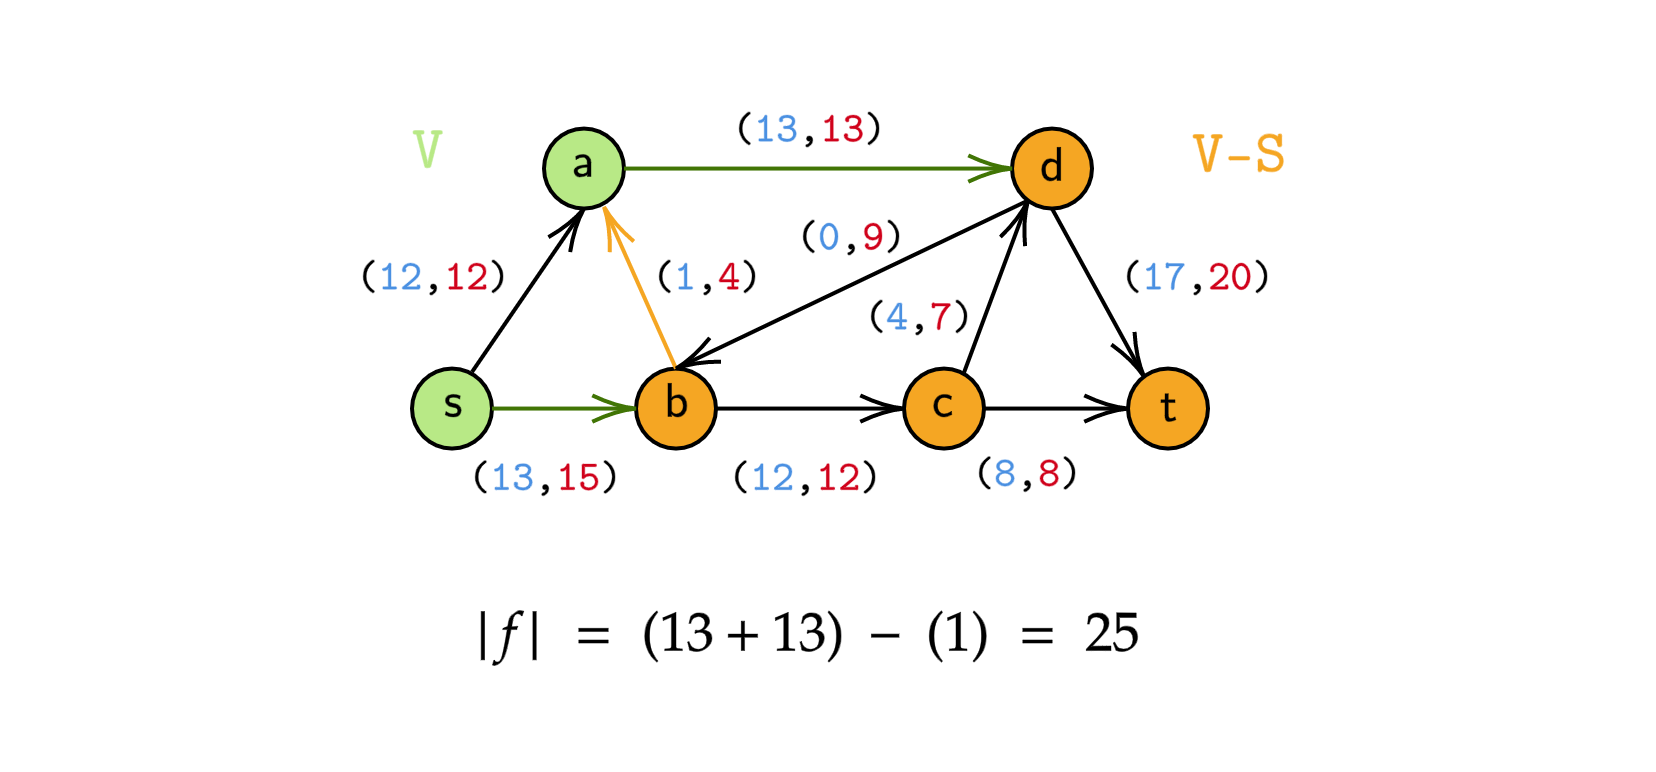
\includegraphics[width=\textwidth]{fig-1.png}
	\end{ex}

	\begin{lem}[Cut Lemma]
		Let $G = (V,A)$ be a directed graph, and suppose that $f$ is an $(s-t)$ flow on $G$. For any $(s-t)$ cut $(S, V - S)$,
		\[|f| = \sum_{a \in \delta^+(S)} f_a - \sum_{a \in \delta^-(S)} f_a\]
	\end{lem}

	\begin{proof}
		The value of $f$ is the amount of flow leaving $s$,
		\begin{align*}
			|f| &= \sum_{a \in \delta^+(s)} f_a \\
					& \text{Since $\delta^-(\{s\}) = \emptyset$,} \\
					&= \sum_{a \in \delta^+(s)} f_a - \sum_{a \in \delta^-(s)} f_a \\
					& \text{By Flow Conservation,} \\
					&= \big(\sum_{a \in \delta^+(s)} f_a - \sum_{a \in \delta^-(s)} f_a \big) + \sum_{v \in S - \{s\}}\big(\sum_{a \in \delta^+(v)} f_a - \sum_{a \in \delta^-(v)} f_a\big) \\
					& \text{Combining the terms to include $s$,} \\
					&= \sum_{v \in S} \big( \sum_{a \in \delta^+(v)} f_a - \sum_{a \in \delta^-(v)} f_a \big) \\
					& \text{Let $a = (i,j) \in A$. There are four cases,}\\
					& \quad \text{1. $(i,j) \in \delta^+(S) \implies f_a$ appears once with coefficient $+1$.} \\ 
					& \quad \text{2. $(i,j) \in \delta^-(S) \implies f_a$ appears once with coefficient $-1$.} \\ 
					& \quad \text{3. $(i,j) \not\in S \implies f_a$ does not appear in the sum.} \\ 
					& \quad \text{4. $(i,j) \in S \implies f_a$ appears twice with coefficients $+1, -1$.} \\ 
					& \text{Consequently,} \\
					&= \sum_{a \in \delta^+(S)} f_a - \sum_{a \in \delta^-(S)} f_a
		\end{align*}
	\end{proof}
		
	\begin{defn}[Cut Capacity]
		\textbf{Capacity} of an $(s-t)$ cut $(S, V - S)$ is,
		\[cap(S) = \sum_{a \in \delta^+(S)} u_a\]
	\end{defn}

	\begin{lem}
		Let $G = (V,A)$ be a directed graph, and suppose that $f$ is an $(s-t)$ flow on $G$. $|f| \leq cap(S)$ for any $(s-t)$ cut $(S, V - S)$.
	\label{lem-ref-1}
	\end{lem}

	\begin{proof}
		By the Cut Lemma,
		\begin{align*}
			|f| &= \sum_{a \in \delta^+(S)} f_a - \sum_{a \in \delta^-(S)} f_a \\
			    &\leq \sum_{a \in \delta^+(S)} f_a \\
			    &= cap(S)
		\end{align*}
	\end{proof}

	\begin{thm}[Maxflow-Mincut]{}
		The maximum value of an $(s-t)$ flow is equal to the minimum capacity of an $(s-t)$ cut.
	\end{thm}

	\begin{proof}
		Let $f^*$ be the flow output by \texttt{Ford-Fulkerson}. Recall that,
		\[S^* = \{v \text{ $|$ } \exists \text{ directed $(s-v)$ path in $G_{f^*}$}\}\]
		\noindent We showed in Lemma \ref{lem-ref-1} that $|f^*| \leq cap(S^*)$, but we can show that $|f^*| = cap(S^*)$. We saw that $\delta^+_{G_{f^*}}(S^*) = \emptyset$ because we could otherwise grow $S^*$. Now, any arc $a \in \delta^+(S^*)$ is not in the residual graph because \texttt{Ford-Fulkerson} requires it to have reached its capacity: $f^*_a = u_a$. Similarly, the reverse of any arc $a \in \delta^-(S^*)$ is not in the residual graph because \texttt{Ford-Fulkerson} requires that $f^*_a = 0$. Now,
		
		\begin{align*}
			|f^*| &= \sum_{a \in \delta^+(S^*)} f_a - \sum_{a \in \delta^-(S^*)} f_a \quad \text{ by the Cut Lemma} \\
			      &= \sum_{a \in \delta^+(S^*)} u_a - \sum_{a \in \delta^-(S^*)} f_a \quad \text{ by Observation 1 above} \\
			      &= \sum_{a \in \delta^+(S^*)} u_a - \sum_{a \in \delta^-(S^*)} 0 \quad \text{ by Observation 2 above} \\
			      &= cap(S^*)
		\end{align*}
	\end{proof}

	\begin{marginfigure}
		$f$ "saturates" the edge $e$ if $f(e) = c(e)$, i.e., $f$ maximizes the flow on $e$. Moreover, if $e$ is not saturated in some maximum $(s-t)$ flow, then $e$ does not occur in any min cut.
		\begin{center}
			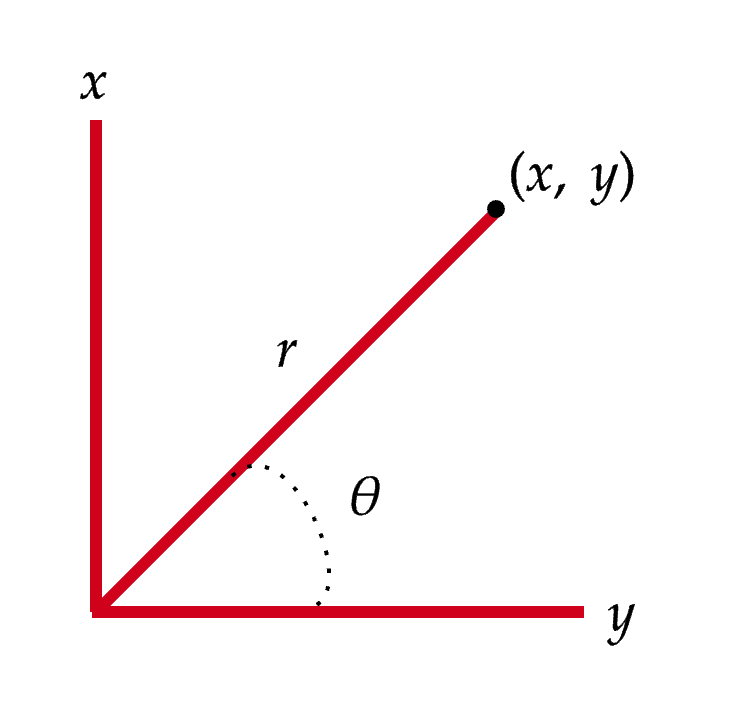
\includegraphics[width=\textwidth]{fig-26.png}
		\end{center}
	\end{marginfigure}

	\begin{rmk}[Running Time]
		\texttt{Ford-Fulkerson} (see Algorithm \ref{fordfulk}) runs in \textbf{pseudo-polynomial time}. Its running time is polynomial in the numeric value of the input, but not in the number of bits required to represent it.
	\end{rmk}

	\begin{proof}
		A single iteration of \texttt{Ford-Fulkerson} runs in $O(m)$ because $G_f$ can be found in $O(m)$, an $(s-t)$ path $P$ can be found in $O(m)$ with Breadth-First Search, and \texttt{Augment} runs in $O(n)$.

		However, the number of iterations is at most $n \cdot U$, where $U$ can be exponential in the input size. The algorithm terminates when $b(P, f) = 0$ for every $(s-t)$ path $P$. Since arc capacities are integral, $b(P,f) \geq 1$. This means that in the worst case, flow is increased by 1 at every iteration. Consequently, the minimum value of any $(s-t)$ cut $C$ satisfies $C \leq n \cdot \max_{a \in A(G)} u_a$. The bound is in terms of $n$, not $m$, because an $(s-t)$ cut separates $V(G)$. Since the flow is at most $n \cdot U$, the number of iterations is bounded by $n \cdot U$.
	\end{proof}

	\begin{ex}{Ford-Fulkerson Running Time Analysis}{label}
		\texttt{Ford-Fulkerson} can take $2U$ iterations on this example,
		\begin{center}
		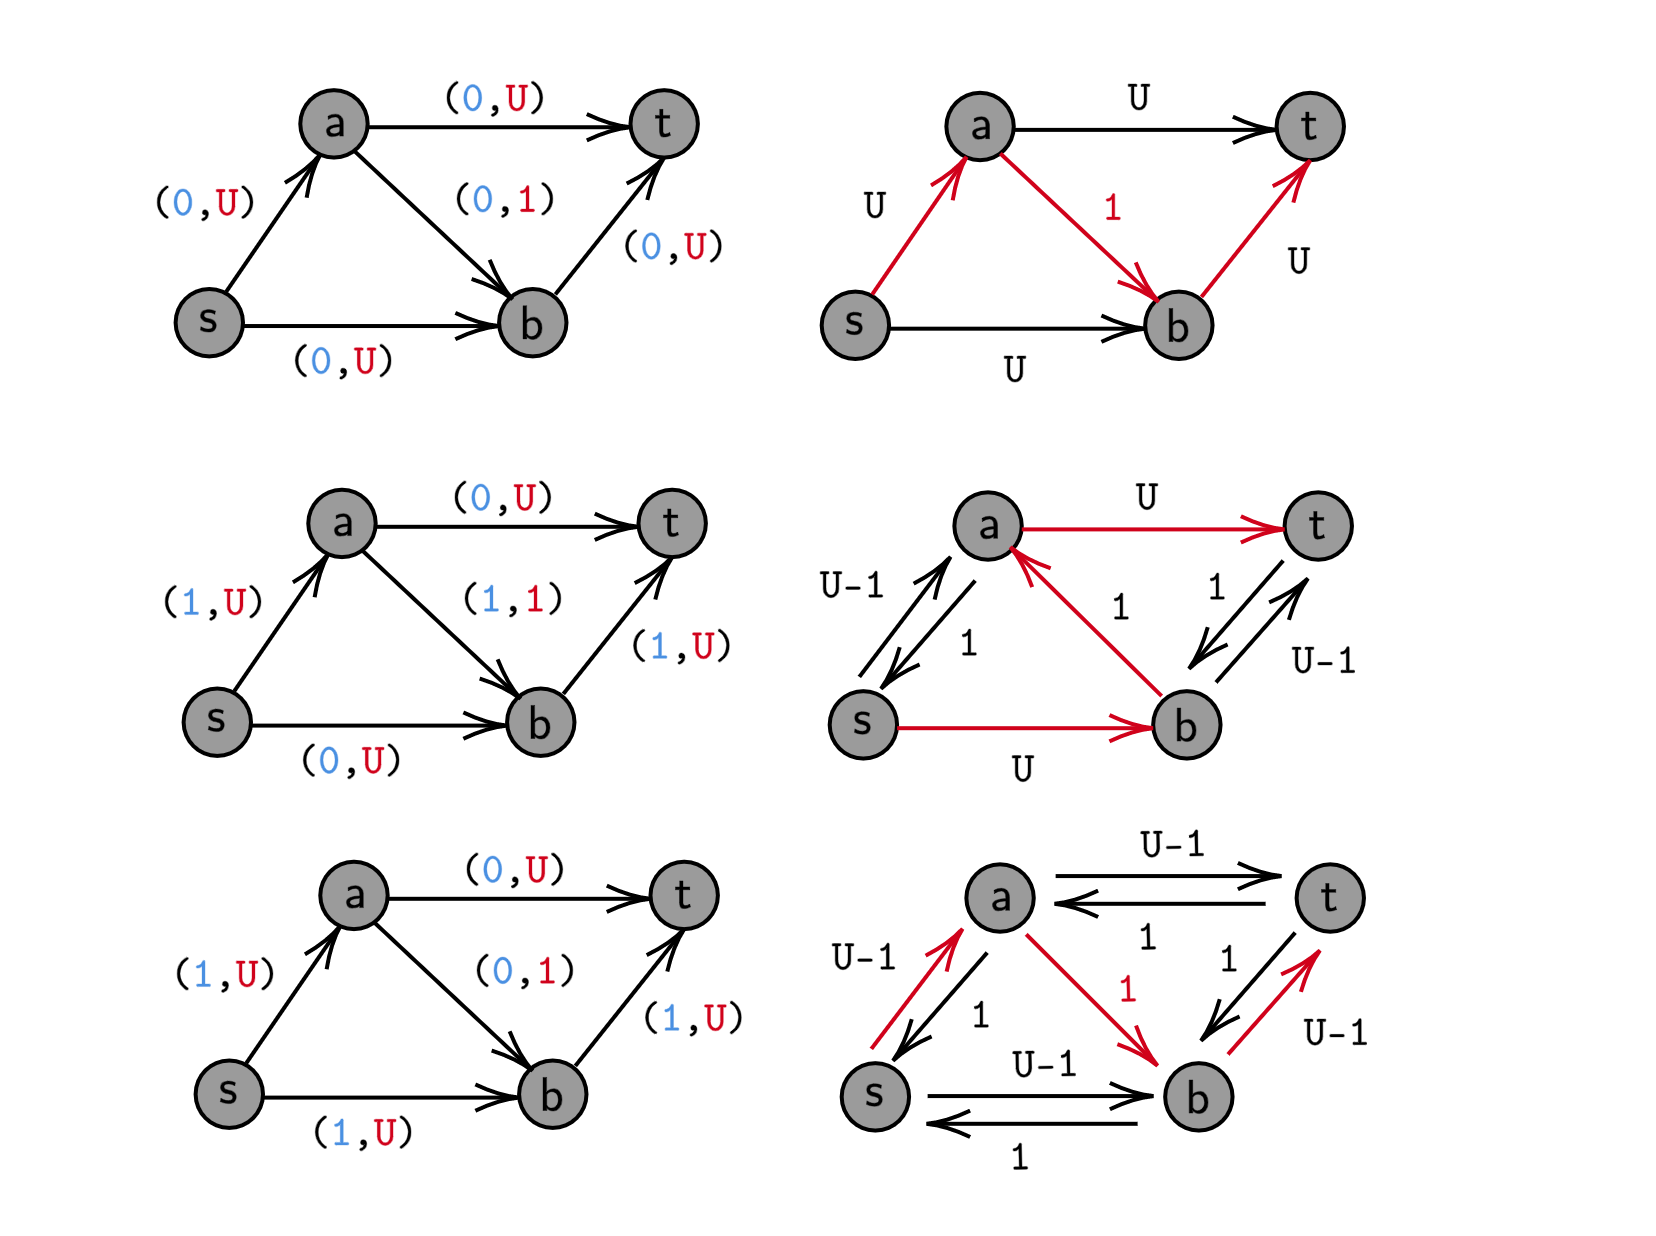
\includegraphics[width=\textwidth]{fig-2.png}
		\end{center}
	\end{ex}

	\subsection{Bipartite Matching Problem}
	\begin{defn}[Independent Set]
 		An \textbf{independent set} is a set of pairwise non-adjacent vertices. The independence number $\alpha(G)$ is the maximal size of an independent set in $G$.
	\end{defn}

	\begin{defn}[Vertex Cover]
 		A \textbf{vertex cover} $X \subset V(G)$ is a set so that every edge of $G$ has an end in $X$. The vertex cover number $\tau(G)$ is the minimum size of a vertex cover in $G$.
	\end{defn}

	\begin{defn}[Matching]
		A \textbf{matching} $M \subset E(G)$ is a set so that every vertex of $G$ is incident to at most one edge of $M$. The matching number $\nu(G)$ is the maximum size of a matching in $G$.
	\end{defn}

	\begin{defn}[Perfect Matching]
		A \textbf{perfect matching} covers $V(G)$.
	\end{defn}

	\begin{defn}[Bipartition]
		A \textbf{bipartition} of a graph $G$ is a pair of subsets $(A, B)$ of $V(G)$ so that $A \cap B = \emptyset$, $A \cup B = V(G)$, and every edge of $G$ has one end in $A$ and another in $B$.
	\end{defn}

	\begin{defn}[Bipartite Matching]
		Let $G = (V, E)$ be an undirected bipartite graph. The \textbf{bipartite matching problem} is the problem of finding $\nu(G)$, the maximum cardinality matching in $G$.
	\end{defn}
 
 	The Ford-Fulkerson Algorithm can be used to solve the bipartite matching problem. To see this, construct an auxiliary network $G = (V, E)$ with bipartition $(X, Y)$ by doing the following,
 	\begin{enumerate}
 		\item Direct each edge $(x_i, y_i)$ from $x_i \rightarrow y_i$
			\item Add a source vertex $s$ with an outgoing arc to each vertex in $X$
			\item Add a sink vertex $t$ with an incoming arc from each vertex in $Y$
			\item Give internal and external arcs capacities of $\infty$ and $1$, respectively\footnote{This is the same as giving every arc a capacity of 1 because the unique arc into each $X$-vertex still has capacity 1}
 	\end{enumerate}

	\begin{ex}{Constructing the Auxiliary Network}{label}
		The auxiliary network for the following bipartite graph is,
		\begin{center}
		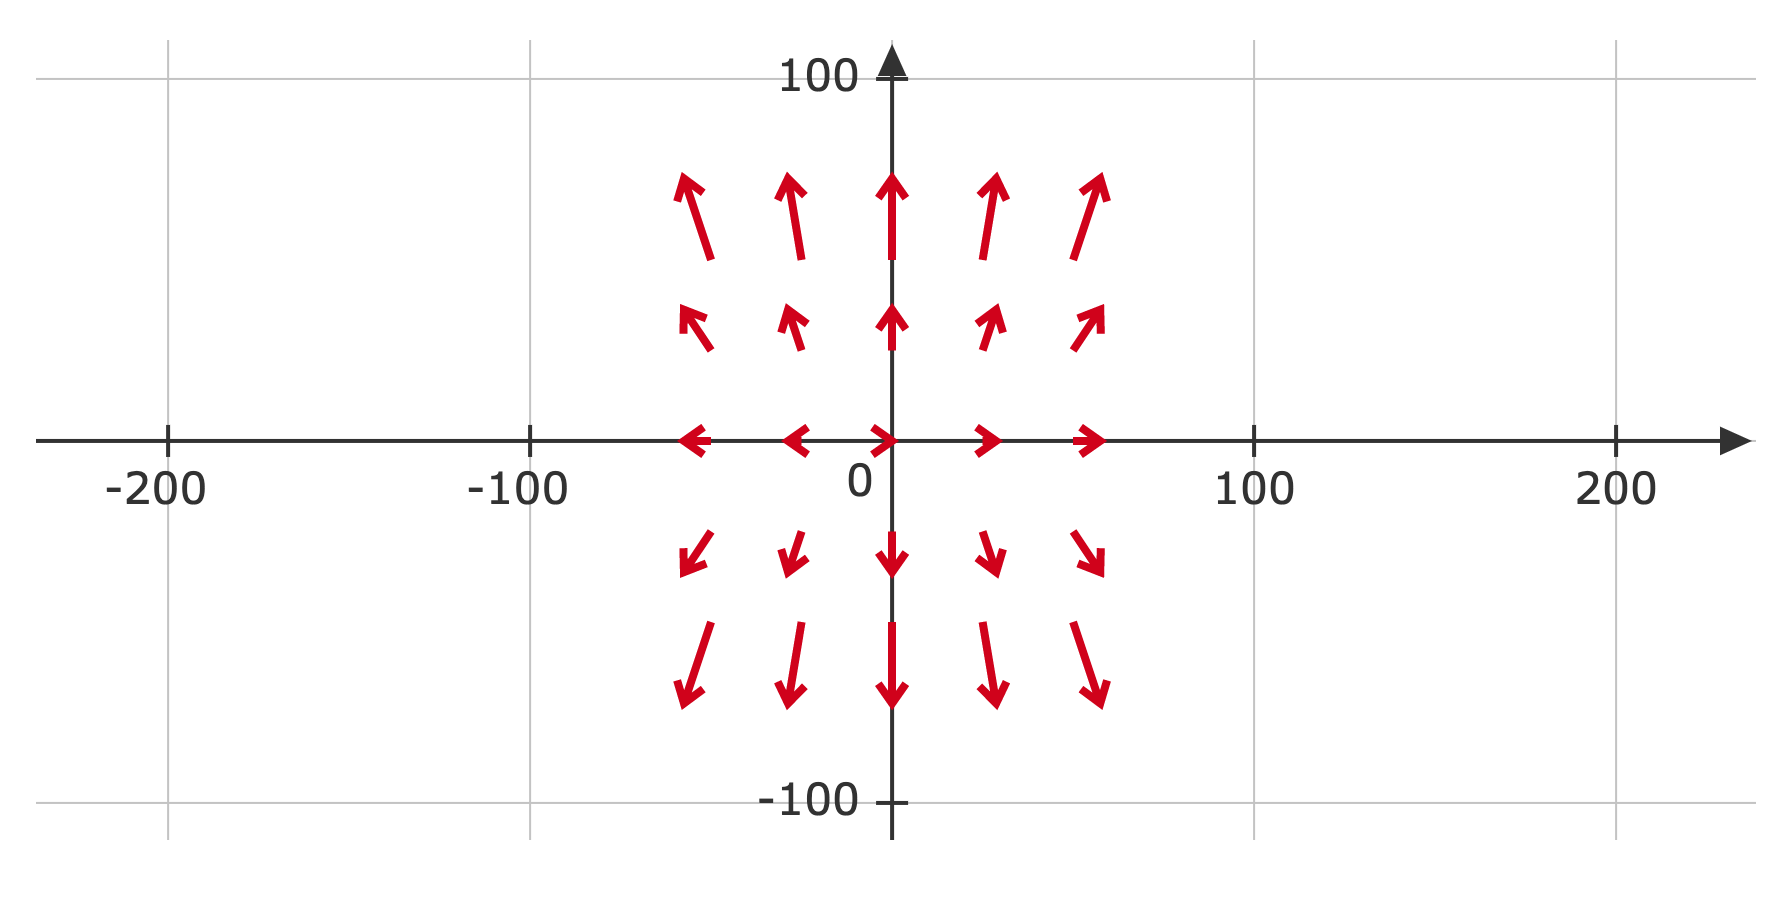
\includegraphics[width=\textwidth]{fig-3.png}
		\end{center}
	\end{ex}

	\begin{thm}[Ford-Fulkerson for Matching]
		There is a polynomial time algorithm to find a maximum cardinality matching in a bipartite graph.
	\end{thm}

	\begin{proof}
		A maximum flow on the auxiliary network is a maximum matching in the original graph. This is because a flow of value $k$ in the auxiliary network consists of $k$ arc-disjoint\footnote{Each arc has capacity 1.} paths, each of which gives an edge in a matching in $G$. Now, since the maximum cardinality of a matching is $\max \{|X|,|Y|\} \leq \frac{n}{2}$, the number of iterations required to run \texttt{Ford-Fulkerson} is at most $n$.
	\end{proof}

	\begin{lem}
		Let $S^*$ be a minimum capacity cut in the auxiliary network of an undirected graph $G$. Every arc in $\delta^+(S^*)$ is of the form $(s, x_i)$ or $(y_j, t)$.
	\end{lem}

	\begin{proof}
		Suppose not. Then $\delta^+(S^*)$ would contain an infinite capacity arc, and so the minimum capacity of a cut in $G$ would be infinite. But the maximum value of a flow on the auxiliary network is $n$ since $s$ has $n$ outgoing arcs, a contradiction.
	\end{proof}

	\begin{thm}[Bipartite Vertex Cover]
		If a vertex cover $C$ and a matching $M$ in a bipartite graph $G$ have the same cardinality, then they are optimal,
		\begin{itemize}
			\item $C$ is a minimum vertex cover
			\item $M$ is a maximum matching
		\end{itemize}
 	\end{thm}

 	\begin{proof}
 		Let $X^* = X \cap S^*$. Then $N(X^*) \subseteq S^* \cap Y$. Otherwise,
 		\[ cap(S^*) = \sum_{a \in \delta^+(S^*)} u_a = \infty \]
 		\noindent $X^* \cup N(X^*) \cup (X - X^*) \cup (N(X - X^*))$ is a partition of $V(G)$. This means that there are three types of edges in $G$,
 		\begin{itemize}
 			\item Edges from $X^*$ to $N(X^*)$
 			\item Edges from $X - X^*$ to $N(X^*)$
 			\item Edges from $X - X^*$ to $Y - N(X^*)$
 		\end{itemize}
 		\noindent We saw above that the fourth type of edge, $X - X^*$ to $N(X^*)$ cannot occur. But then $X - X^* \cup N(X^*)$ is a vertex cover and its cardinality is the capacity of the $(s-t)$ cut.
 	\end{proof}

 	\begin{cor}
 		There is a polynomial time algorithm to find a minimum cardinality vertex cover in a bipartite graph.
 	\end{cor}

 	\subsection{Extensions to Maximum Flow}
 		\begin{defn}[Circulations with Demands]
 		Let $G = (V, A)$ be a directed graph. We associate a demand $d_v$ for flow with each node\footnote{If $d_v < 0$, this indicates that $v$ has supply of $-d_v$. If $d_v = 0$, then the node is neither a source nor a sink.},
 		\begin{itemize}
 			\item $S = \{s_1, \dots, s_k\}$ is the set of sink nodes with positive demand
 			\item $T = \{t_1, \dots, t_l\}$ is the set of source nodes with negative demand
 			\item $s$ is a super-source with arcs $(s,s_i)$ and capacities $d_{s_i}$ for all $s_i \in S$
 			\item $t$ is a super-sink with arcs $(t_j, t)$ and capacities $-d_{t_j}$ for all $t_j \in T$
 		\end{itemize}
 		\noindent A \textbf{circulation with demands} $f: A(G) \rightarrow \{0\} \cup \mathbb{R}^+$ satisfies,
 		\begin{itemize}
 			\item $0 \leq f_a \leq u_a$ for all $a \in A(G)$
 			\item $\sum_{a \in \delta^-(v)} f_a - \sum_{a \in \delta^+(v)} f_a = d_v$ for all $v \in V(G) - \{s,t\}$
 		\end{itemize}
 		\noindent There exists a feasible circulation to the multi-source supply and demand problem if and only if there is a flow from $s$ to $t$ of value $\sum_{v:d_v > 0} d_v = 0$.
 	\end{defn}

	\begin{defn}[Circulations with Demands and Lower Bounds]
 		Let $G = (V, A)$ be a directed graph. We associate a lower bound $l_a = l_{ij}$ on each arc $a = (i,j)$, where $0 \leq l_a \leq u_a$. A \textbf{circulation with demands and lower bounds} can be reduced to one without lower bounds,
 		\begin{itemize}
 			\item $l_e \leq f_a \leq u_a \iff 0 \leq f_a \leq u_a - l_a$ for all $a \in A(G)$
 			\item $d_v^* = d_v + \sum_{(k,v) \in A} l_{kv} - \sum_{(v,k) \in A} l_{vk}$ for all $v \in V(G)$
 		\end{itemize}
 	\end{defn}

 	 	\begin{ex}{Airline Scheduling}{label}
 	 	\begin{tabular}{ll}
			\textbf{\texttt{Origin and Destination}} & \textbf{\texttt{Time}} \\
			\texttt{Boston - San Francisco} & \texttt{7am - 9am} \\
			\texttt{Toronto - Boston} & \texttt{7am - 8am}
		\end{tabular}

		\vphantom{.}

 		We create a network flow as follows,
 		\begin{itemize}
 			\item $o_i$ is a vertex representing the origin of flight $i$
 			\item $d_i$ is a vertex representing the destination of flight $i$
 			\item $s$ is a source vertex with supply $k$
 			\item $t$ is a sink vertex with demand $k$
 			\item $(d_i, t)$ has capacity 1 for every flight $i$
 			\item $(d_i, o_j)$ has capacity 1 if flight $i$ can be serviced after flight $j$
 			\item $(o_i, d_i)$ has a lower bound of 1
 		\end{itemize}
 		There is a way to perform all flights using at most $k$ planes $\iff$ There is a feasible circulation in our network.
	\end{ex}

	\begin{ex}{Open-Pit Mining}{label}
		We are given that,
		\begin{itemize}
			\item $V$ is a set of blocks, each of which generates a profit $\pi_i$
			\item 3 upper neighbors must be removed to dig block $i$
		\end{itemize}
		\noindent We create a network flow as follows,
		\begin{itemize}
			\item $v_i \in V$ represents block $i$ in our pit
			\item $s$ and $t$ are the source and sink vertices
			\item $(s,v_i)$ has capacity $\pi_i$ if and only if $\pi_i > 0$
			\item $(v_i, t)$ has capacity $|\pi_i|$ if and only if $\pi_i < 0$
			\item Infinite capacity arcs exist between $i$ and its 3 neighbors
		\end{itemize}

		We know that $cap(S^*)$ is finite because,
		\[cap(\{s\})= \sum_{i:\pi_i > 0} \pi_i\]
		is finite by construction. The capacity of the an $(s-t)$ cut $S$ is,
		\begin{align*}
			cap(S) &= \sum_{a \in \delta^+(S)}  u_a \\
			       &= \sum_{i \not\in S: \pi_i > 0} \pi_i + \sum_{i \in S: \pi_i > 0} |\pi_i| \\
			       &= \bigg(\sum_{i \in V: \pi_i > 0} \pi_i - \sum_{i \in S: \pi_i > 0} \pi_i \bigg) + \sum_{i \in S: \pi_i > 0} |\pi_i| \\
			       &= \bigg(\sum_{i \in V: \pi_i > 0} \pi_i - \sum_{i \in S: \pi_i > 0} \pi_i \bigg) - \sum_{i \in S: \pi_i > 0} \pi_i \\
			       &= \underbrace{\sum_{i \in V: \pi_i > 0} \pi_i}_{constant} - \sum_{i \in S} \pi_i
		\end{align*}
		Minimizing $cap(S)$ solves the open-pit mining problem, since it requires us to maximize the profit associated with $S$.
	\label{mining}
	\end{ex}

	\begin{ex}{Image Segmentation}{label} 
 		We create a network flow as follows,	
 		\begin{itemize}
 				\item $v_i$ is a vertex representing the pixel $i$
 				\item $s$ is a source vertex representing the foreground
 				\item $t$ is a sink vertex representing the background
 				\item $f_i$ is the likelihood that the pixel $i$ is in the foreground
 				\item $b_i$ is the likelihood that the pixel $i$ is in the background
 				\item $\rho_{ij}$ is a penalty for separating adjacent pixels $i$ and $j$
 				\item $(s, v_i)$ has capacity $f_i$
 				\item $(v_j, t)$ has capacity $b_j$
 				\item $(v_i,v_j)$ and $(v_j,v_i)$ have capacity $\rho_{ij}$
 		\end{itemize}

 		The capacity of the an $(s-t)$ cut $S$ is,
 		\begin{align*}
 			cap(S) &= \sum_{a \in \delta^+(S)}  u_a \\
 			       &= \sum_{i \not\in S} f_i + \sum_{j \in S} b_j + \sum_{(i,j) \in \delta^+(S)} \rho_{ij} \\
 			       &= \big(\sum_{i \in V} f_i - \sum_{i \in S} f_i\big) + \big(\sum_{j \in V} b_j - \sum_{j \not\in S} b_j\big) + \sum_{(i,j) \in \delta^+(S)} \rho_{ij} \\
 			       &= \underbrace{\sum_{i \in V}(f_i + b_i)}_{constant} - \sum_{i \in S}f_i - \sum_{j \not\in S}b_j + \sum_{(i,j) \in \delta^+(S)} \rho_{ij}
 		\end{align*}

 		Minimizing $cap(S)$ is solves the segmentation problem,
 		\[ \max_S \sum_{i \in S}f_i + \sum_{j \not\in S} b_j - \sum_{(i,j) \in \delta^+(S)} \rho_{ij}\]
 		\begin{itemize}
 			\item There is a bonus $f_i$ if pixel $i$ is placed in the foreground
 			\item There is a bonus $b_j$ if pixel $j$ is placed in the background
 			\item There is a penalty $\rho_{ij}$ for separating pixels $i$ and $j$
 		\end{itemize}
 	\end{ex}

 	\subsection{Flow Decomposition Theorem}
 	\begin{marginfigure}
	\textbf{Recap on Flow Decomposition:}

	\noindent Let $G = (V, A)$ be a directed graph and suppose that $f$ is an $(s-t)$ flow of value $k$. Then there exist directed paths $P_1, \dots, P_k$ (possibly repeated) from $s$ to $t$ in $G$, and every edge belongs to at most $f(e)$ paths.
	\end{marginfigure}

	\begin{lem}
		Let $G = (V, A)$ be a directed graph and suppose that $f$ is an $(s-t)$ flow of value $k > 0$ Then $f$ contains a path or a cycle.
	\label{fdtlemma}
	\end{lem}

	\begin{proof}
		If $f$ contains a directed cycle $C$, then we are done. Assume that this is not the case. Since $k > 0$,
		\[ \sum_{a \in \delta^+(\{s\})}f_a \geq 1\]
		\noindent so there is at least one arc $a_1 = (s, v_1)$ with $f_{a_1} \geq 1$. By flow conservation, there exists an arc $a_2 = (v_1, v_2)$ ($v_2 \neq s$ since the flow is acyclic). Repeating inductively, we can construct an $(s-t)$ path with $\min_{a \in P}f_a \geq 1$.
	\end{proof}

	\begin{thm}[Flow Decomposition Theorem]
		Let $G = (V, A)$ be a directed graph and suppose that $f$ is an $(s-t)$ flow of value $k > 0$. Then $f$ can be decomposed into at most $m$ $(s-t)$ paths and directed cycles.
	\end{thm}

	\begin{proof}
		We proceed by induction on the number of arcs in the graph.
		\begin{itemize}
			\item (Base Case) If $m = 0$, then $f$ is empty and trivially consists of zero paths and cycles. If $m = 1$, then $f$ is a single arc $(s,t)$ and thus can be decomposed into one $(s,t)$ path.
			\item (Induction Hypothesis) Assume that any flow with $k < m$ arcs can be decomposed into a collection of at most $k$ cycles and $(s-t)$ paths. Consider a flow $f$ with $m$ arcs. By Lemma \ref{fdtlemma}, $f$ contains a path or a cycle. There are two cases,
			\begin{enumerate}
				\item If $f$ contains a cycle $C$, then let $f^*$ be the flow obtained by removing $\min_{a \in C}f_a$ units of flow from each arc in $C$. Then $f^*$ has at least one fewer arc than $f$. By the induction hypothesis, $f^*$ decomposes into at most $m-1$ paths and cycles. Thus, $f$ decomposes into at most $m$ paths and cycles.
				\item If $f$ contains a path $P$, then let $f^*$ be the flow obtained by removing $\min_{a \in C}f_a$ units of flow from each arc in $P$. Proceed as in Case 1 to decompose $f^*$ into $m-1$ paths and cycles.
			\end{enumerate}
		\end{itemize}		
	\end{proof}

	\begin{cor}
		The Ford-Fulkerson algorithm can terminate in $m$ iterations.
	\end{cor}

	\subsection{Fast Flow Algorithms}
	\begin{rmk}
		Let $G = (V, A)$ be a directed graph and suppose that $f^*$ is an maximum $(s-t)$ flow on $G$. Then there is a path $P$ in $G$ with,
		\[u_P \geq \frac{1}{m}|f^*|\]
	\end{rmk}

	\begin{proof}
		By the Flow Decomposition Theorem, $f^*$ consists of at most $m$ paths. Thus, at least one of these paths carries $\frac{1}{m}|f^*|$ flow.
	\end{proof}

	\begin{rmk}
		Let $G = (V, A)$ be a directed graph and suppose that $f^*$ is an maximum $(s-t)$ flow on $G$. Let $f$ be any other $(s-t)$ flow on $G$. Then,
		\[b(P, f) \geq \frac{|f^*|-|f|}{m}\]
		\noindent for some path in the residual graph $G_f$.
		\label{observ1}
	\end{rmk}

	\begin{proof}
		$f^* - f$ satisfies the flow conservation constraints. By the Flow Decomposition Theorem, $f^* - f$ can be decomposed into at most $2m$ paths and cycles. Only one direction of each arc is used, so we can assume that $(f^*-f)$ can be decomposed into at most $m$ paths. Thus, at least one of these paths carries $\frac{|f^*|-|f|}{m}$.
	\end{proof}

	\begin{defn}[Maximum Capacity]
		The \textbf{maximum capacity augmenting path algorithm} chooses augmenting paths greedily by capacity.
	\end{defn}

	\begin{marginfigure}
		\textbf{(Recap)} $1 - x < e^{-x}$ for all $x \neq 0$.
	\end{marginfigure}
	
	\begin{thm}
		The maximum capacity augmenting path algorithm terminates in at most $m \cdot (\ln n + \ln U)$ iterations\footnote{Weakly polynomial algorithms depend on the size of the input.}, where $U = \max_{a \in A}u_a$.
	\end{thm}

	\begin{proof}
		Suppose that the algorithm finds paths $\{P_1, P_2, \dots, P_T\}$. We need to show that $T \leq m \cdot (\ln n + \ln U)$. Denote by $f_t$ the flow after $t$ iterations. By Remark \ref{observ1}, the path $P_{t+1}$ satisfies,
		\[b(P_{t+1}, f_t) \geq \frac{|f^*|-|f_t|}{m} := \frac{\triangle_{t+1}}{m}\]
		\noindent $\triangle_{t+1}$ is the flow quantity that remains to be found at step $t+1$. In particular, $\triangle_{t+1} \leq \triangle_t - \frac{1}{m}\cdot \triangle_t$ since we fall by $\frac{1}{m}$ at each iteration. Continuing inductively, we get that $\triangle_{t+1} \leq (1 - \frac{1}{m})^t \cdot \triangle_1 = (1 - \frac{1}{m})^t \cdot |f^*|$. But then, $\triangle_{t+1} \leq e^{-\frac{t}{m}} \cdot |f^*|$. Setting $t = m \cdot ln|f^*|$,
		\[\triangle_{t+1} < e^{-\frac{m \cdot ln|f^*|}{m}} |f^*| = 1\]
		\noindent After $T=m \cdot \ln|f^*|$ steps, the quantity of flow remaining to be found is less than one. Flows are integral, so we have found $|f^*|$. Since the maximum cut in $G$ has value $n\cdot U$, $\ln|f^*| \leq \ln u \cdot U = \ln u + \ln U$. Thus, the number of iterations is at most $m \cdot (\ln u + \ln U)$.
	\end{proof}

	\begin{algorithm}
	  \caption{Maximum Capacity Augmenting Paths}\label{greedyaug}
	  \Comment{$f$ is globally given, and initially set to $0$.}
	  \Comment{$\texttt{Augment}(P,f)$ is globally given}
	  \Function{Ford-Fulkerson($G$)}{
	  	\ForEach{$a \in A(G)$}{
	  		$f(a) \assign 0$\;
	  		$G_f \assign \text{residual network of $G$ with respect to $f$}$;
	  	}
	  	\While{$\exists (s-t) \text{ path $P$ in $G_f$}$}{
	  		$P^* \assign \text{maximum capacity augmenting path}$
	  		$f \assign \FuncCall{Augment}{$P^*$, $f$}$\;
	  		$\text{Update $G_f$}$;
	  	}
	    \Return{$f$}\;
	  }
	\end{algorithm}

	\begin{thm}
		The maximum capacity augmenting path algorithm takes $O(m^2)$ time per iteration. Binary search reduces it to $O(m \cdot \log m)$.
	\end{thm}

	\begin{proof}
		Label the arcs in $G_f$ by \{1, 2, \dots, 2m\} in decreasing order of residual capacity. We can test if there is an $(s-t)$ path that uses arcs $\{1, \dots k\}$ in $O(m)$ time by Breadth-First Search. Repeating this process for all $k$ gives a total time in $O(m^2)$.
	\end{proof}

	\begin{cor}
		It total, the algorithm runs in $O(m^3 \cdot (\ln u + \ln U))$ time.
	\end{cor}

	\begin{defn}[Shortest Length]
		The \textbf{shortest length residual path algorithm} chooses augmenting path greedily by length\footnote{The length of a path is the number of arcs comprising it.}.
	\end{defn}

	\begin{marginfigure}
		\textbf{The Potential Function Argument:}

		If $\phi$ satisfies,
		\begin{itemize}
			\item $\phi$ decreases at a rate of $\delta$
			\item $\phi$ is lower bounded by $\ell$
		\end{itemize}
		\noindent Then $\phi$ becomes fixed at time $T$. Given the starting value $\phi_0$ and $\ell$, we know that $\phi$ becomes fixed at $-\phi_0*|\delta| = \phi$.
	\end{marginfigure}

	\begin{rmk}
		An iteration of the shortest length augmenting path algorithm is in $O(m)$ if the shortest $(s-t)$ paths are found with Breadth-First Search.
	\end{rmk}

	\begin{thm}
		The shortest length augmenting path algorithm terminates in at most $m \cdot n$ iterations. This puts its runtime in $O(m^2 \cdot n)$.
	\end{thm}

	\begin{proof}
		Suppose that the algorithm finds paths $\{P_1, P_2, \dots, P_T\}$. We need to show that $T \leq m \cdot n$. Let $f_t$ be the flow after $t$ iterations, and consider its residual graph $G_{f_t}$. Define $d_t(v)$ as the distance of a vertex $v$ from the source $s$ in $G_{f_t}$, and consider $\phi_t = \sum_{v \in V} d_t(v)$. We will use a potential energy function argument to show that,
		\[d_t(u) \leq d_{t+1}(u) \quad \text{for all $t$}\]
		
		\noindent If $t = 0$, then $\phi_0 = \sum_{v \in V} d_0(v) \geq 0$ since $d_0$ is a distance. Moreover, $d_t(v) \leq n - 1$ since $G$ has $n$ vertices. This means that,
		\[\phi_t = \sum_{v \in V}d_t(v) \leq n^2\]

		\noindent To apply the argument, we need to prove that $\phi_t$ is non-decreasing. It suffices to show that $d_t(v)$ is non-decreasing for each vertex $v$. Suppose not. Then there exists $t \in \mathbb{N}$ and a vertex $v \in V(G)$ such that $d_t(v) > d_{t+1}(v)$. Consider the closest such vertex to $s$. Let $u$ be the vertex preceding it on the shortest path from $s$ to $v$ in $G_{f_{t+1}}$. Then $d_{t+1}(v) = d_{t+1}(u) + 1$ and $d_t(u) \leq d_{t+1}(u)$.
		\begin{itemize}
			\item If $(u,v) \in G_{f_t}$, then,	
			\begin{align*}
				d_t(v) &\leq d_t(u) + 1 \text{\phantom{ since $P_t$ is the shortest path in $G_{f_t}$}}\\
							 &\leq d_{t+1}(u) + 1 \text{ since $d_t(u) \leq d_{t+1}(u)$} \\
							 &= d_{t+1}(v) \text{ since $d_{t+1}(v) = d_{t+1}(u)+1$} \\
							 &< d_{t+1}(v) \text{ since $d_t(v) > d_{t+1}(v)$} \\
							 &\text{a contradiction.}
			\end{align*}
			\item If $(u,v) \not\in G_{f_t}$, $(v,u) \in P_t$ since $(u,v) \in G_{f_{t+1}}$. But,
			\begin{align*}
				d_t(u) &= d_t(v) + 1 \text{ since $P_t$ is the shortest path in $G_{f_t}$} \\
						   &> d_{t+1}(v) + 1 \\ 
						   &= d_{t+1}(u) + 2 \text{ since $d_{t+1}(v) = d_{t+1}(u)+1$} \\
						   &\geq d_t(u) + 2 \\
						   &\text{a contradiction.}
			\end{align*}
		\end{itemize}

		\noindent $P_t$ is augmented by its bottleneck capacity, and there is at least one arc $a_t$ with that capacity. It suffices to prove that each arc can be the bottleneck arc at most $\frac{n}{2}$ times\footnote{This argument works because we have proven that $\phi$ is a bounded function.}, because this means that the number of iterations is at most $2m \cdot \frac{n}{2} = mn$.
	\end{proof}

	\begin{lem}
		Each arc can be the bottleneck arc at most $\frac{n}{2}$ times.
	\end{lem}

	\begin{proof}
		Let $(u,v) \in A(G_{f_t})$ be the bottleneck arc in the augmenting path $P_t$. Since $P_t$ is the shortest $(s-t)$ path in $G_{f_t}$, we have that $d_t(v) = d_t(u) + 1$. Now, $(u,v) \not\in G_{f_{t+1}}$ since $(u,v)$ is the bottleneck arc in iteration $t$. Suppose that $(u,v)$ is a bottleneck in iteration\footnote{$(u,v)$ cannot be a bottleneck at iteration $t + 1$ because it is not in the residual graph $G_{f_{t+1}}$.} $t + 1 + k > t + 1$ ($k > 0$). Then $(u,v)$ must have been added back into the residual graph $G_{f_{t + 1 + k}}$. This means that the reverse arc $(v,u)$ must have been used at some time $t + 1 \leq t^{\prime} < t + 1 + k$. As $P_{t^{\prime}}$ is the shortest $(s-t)$ path in $G_{f_{t^{\prime}}}$, we have:
		\begin{align*}
			d_{t^{\prime}}(u) &= d_{t^{\prime}}(v) + 1 \\
			&\geq d_t(v) + 1\\
			&= d_t(u) + 2
		\end{align*}
		\noindent Since the distance label of $u$ must have increased by at least 2, this can happen at most $\frac{n}{2}$ times. Otherwise, we get that $d_t(u) > n$.
	\end{proof}

		\begin{algorithm}
	  \caption{Shortest Length Augmenting Paths}\label{greedyaug}
	  \Comment{$f$ is globally given, and initially set to $0$.}
	  \Comment{$\texttt{Augment}(P,f)$ is globally given}
	  \Function{Ford-Fulkerson($G$)}{
	  	\ForEach{$a \in A(G)$}{
	  		$f(a) \assign 0$\;
	  		$G_f \assign \text{residual network of $G$ with respect to $f$}$;
	  	}
	  	\While{$\exists (s-t) \text{ path $P$ in $G_f$}$}{
	  		$P^* \assign \text{shortest length augmenting path}$
	  		$f \assign \FuncCall{Augment}{$P^*$, $f$}$\;
	  		$\text{Update $G_f$}$;
	  	}
	    \Return{$f$}\;
	  }
	\end{algorithm}